% --------------------------------------------------------------------------- %
% !TEX encoding = UTF-8
% !TEX TS-program = pdflatex
% !TEX root = main.tex
% !TEX spellcheck = en-EN
% --------------------------------------------------------------------------- %
\chapter{Results}
%	In this chapter the main results obtained using the procedure and the code proposed in \chref{ch: Estimation} will be analyzed and discussed. The results are divided in three different test cases. The first provides a verification of the code: it utilize a totally artificial dataset to ensure that the program is capable of retrieving the correct information \textit{hidden} in the dataset. The second 
	
	
	
	
	
	
	
	
	
	
	
	
	
	
	
	
	
	\section{Test case 1 - Code Verification}
		Verification with totally artificial data set
		\begin{itemize}
			\item 1 parameter (\fref{val: 1paramData}, \ref{val: 1param1}, \ref{val: 1param2}, \ref{val: 1param3})
			\item 2 parameters (\fref{val: 2paramData}, \ref{val: 2param1}, \ref{val: 2param2})
		\end{itemize}
	
		\begin{figure}
			\centering
			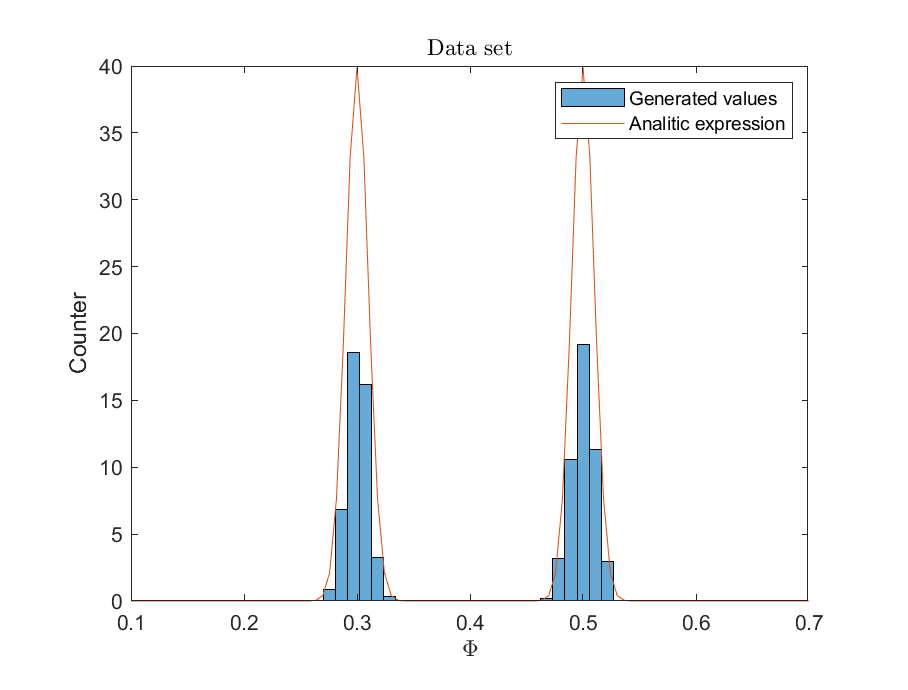
\includegraphics{validation/1paramData.eps}
			\caption{}
			\label{val: 1paramData}
		\end{figure}
		\begin{figure}
			\centering
			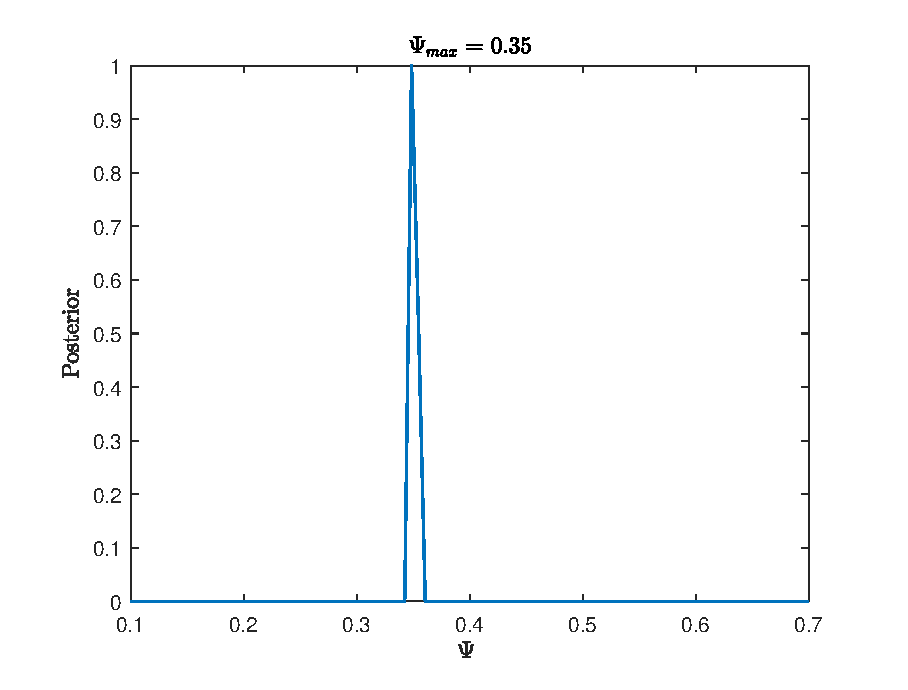
\includegraphics{validation/1param1.eps}
			\caption{}
			\label{val: 1param1}
		\end{figure}
		\begin{figure}
			\centering
			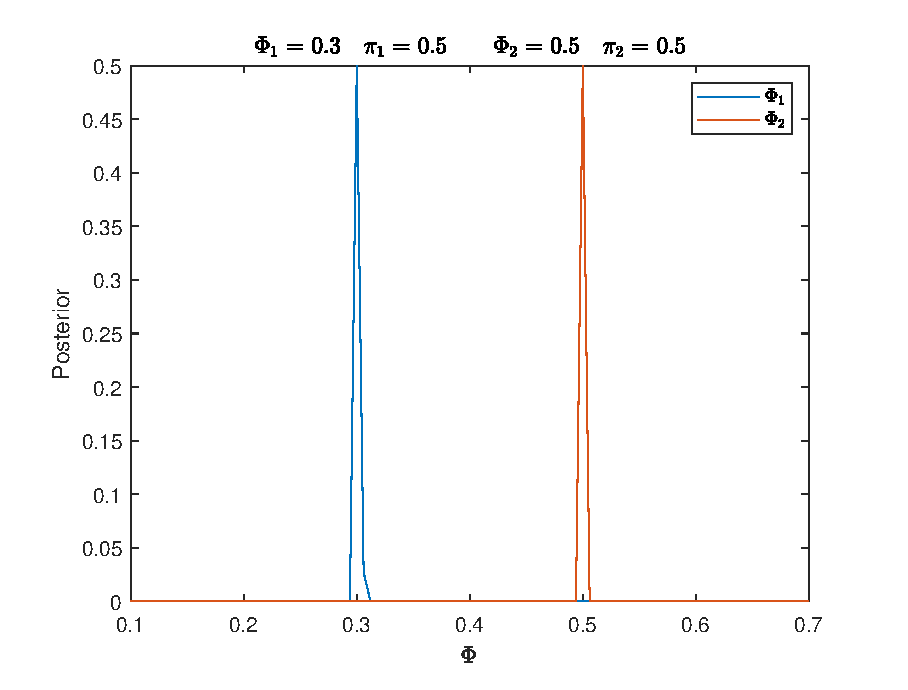
\includegraphics{validation/1param2.eps}
			\caption{}
			\label{val: 1param2}
		\end{figure}
		\begin{figure}
			\centering
			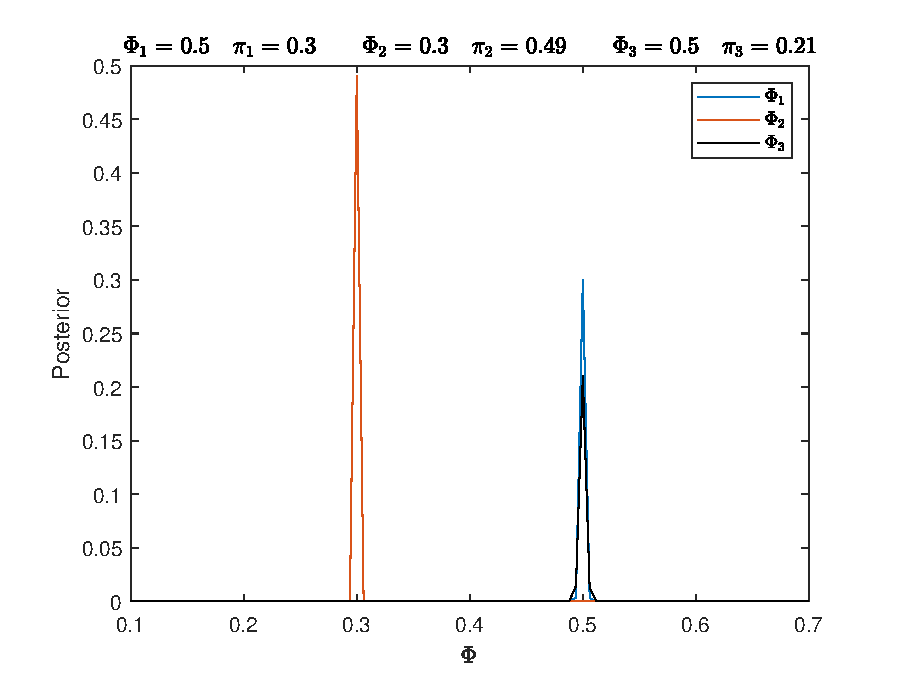
\includegraphics{validation/1param3.eps}
			\caption{}
			\label{val: 1param3}
		\end{figure}

		\begin{figure}
			\centering
			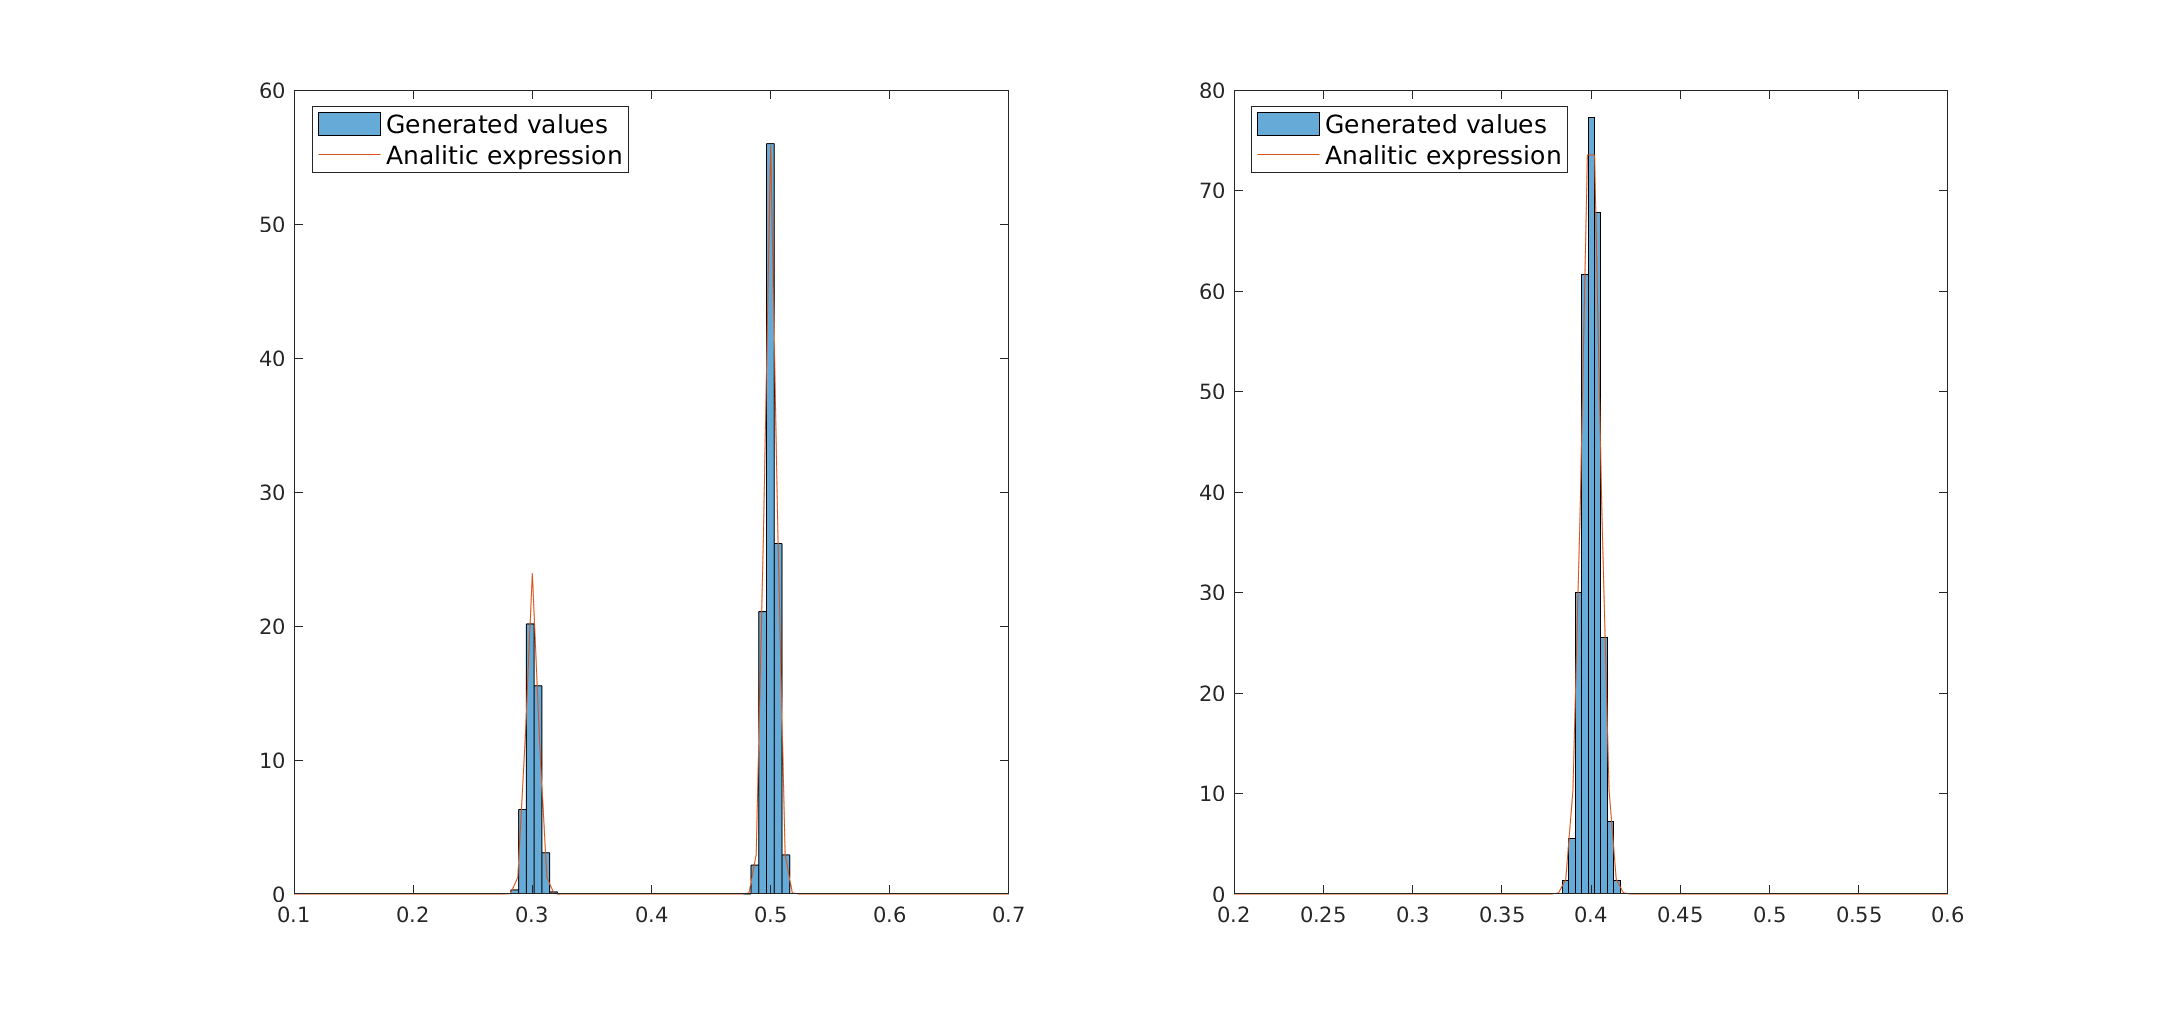
\includegraphics[width=\linewidth]{validation/2paramData.eps}
			\caption{}
			\label{val: 2paramData}
		\end{figure}
		\begin{figure}
			\centering
			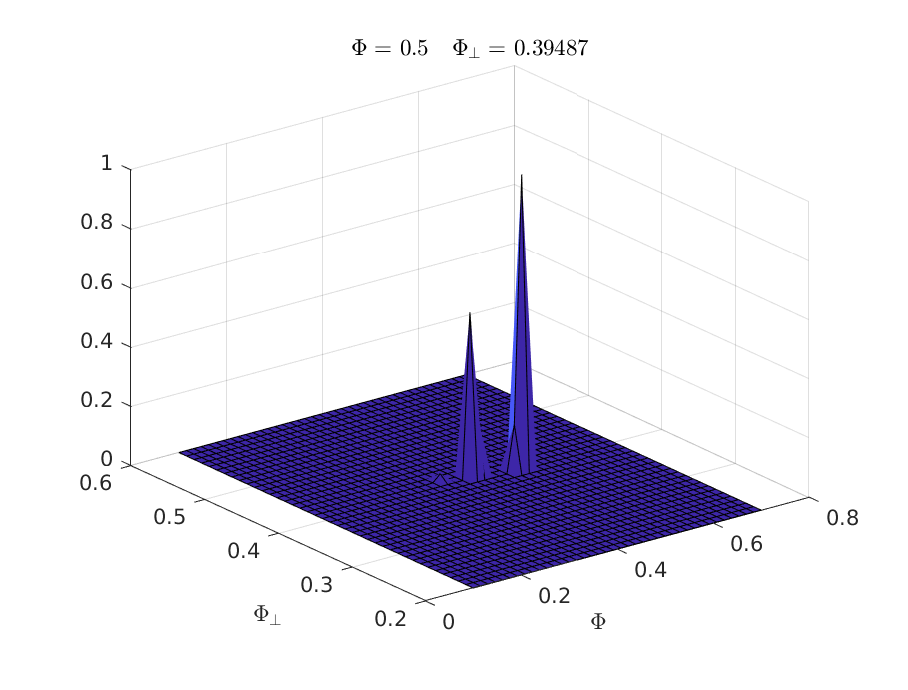
\includegraphics[width=\linewidth]{validation/2param1.eps}
			\caption{}
			\label{val: 2param1}
		\end{figure}
		\begin{figure}
			\centering
			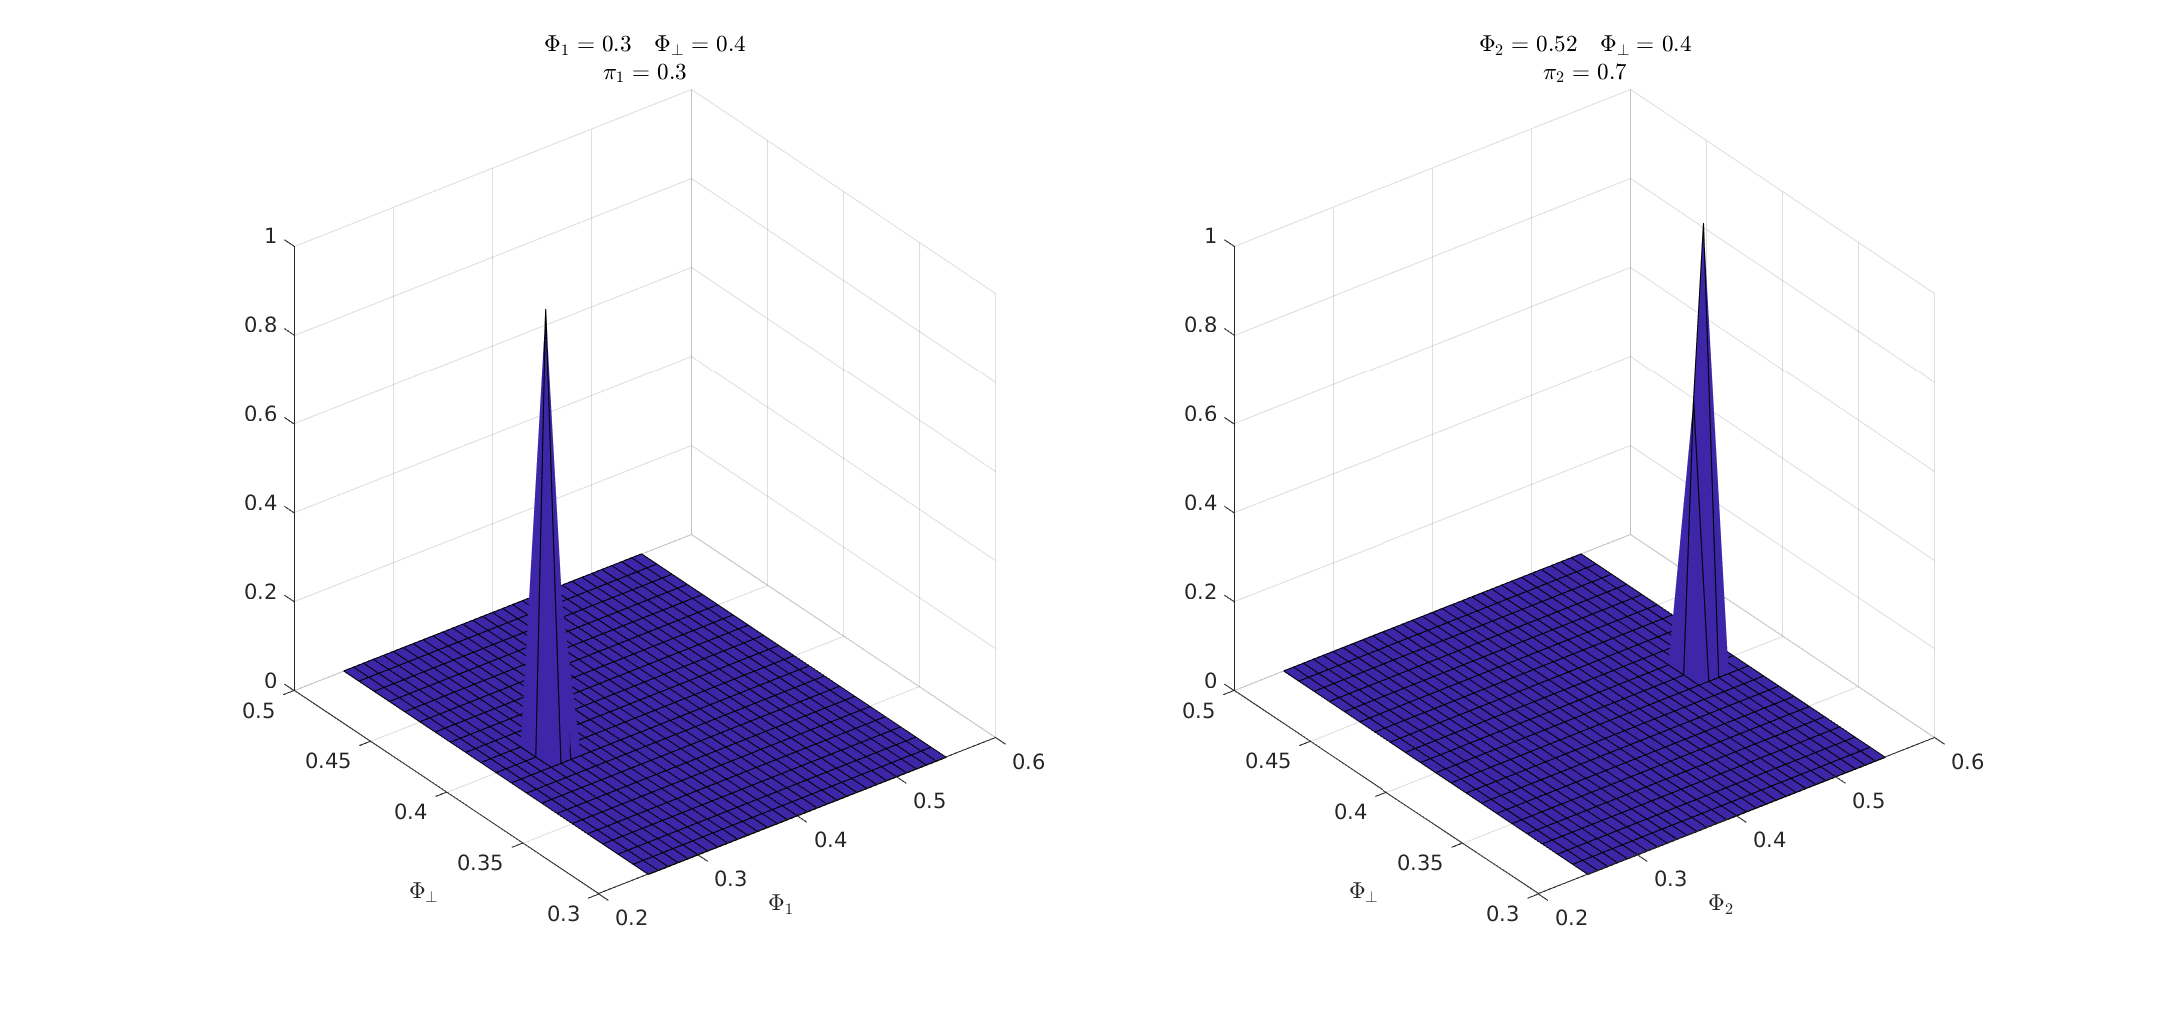
\includegraphics[width=\linewidth]{validation/2param2.eps}
			\caption{}
			\label{val: 2param2}
		\end{figure}

	\section{Test case 2 - Experimental Dataset}
		Brief description of the available experimental campaigns (Brandes + other 2 references) and their limitations.
	
		\subsection{Brandes Experimental campaign}
		Description of the Brandes results and impossibility to use the raw data
		
		\subsection{Data Set generation}
		Generation of an artificial data set starting from the relations discovered by Brandes. The dependency on the diameter distribution is not taken into account as it can be retrieved a posteriori.
	
		\subsection{Application to the Brandes data set}
		\begin{itemize}
			\item Example for 1 diameter interval
			\item Shape parameters - diameter distribution (Work in progress)
		\end{itemize}
		
	\section{Test case 3 - Let it snow!}
		Falling snow test case (Check the terminal velocity distribution) with PoliDrop
